%!TEX root = project.tex

\chapter*{About this project}
\paragraph{Abstract}
A brief description of what the project is, in about two-hundred and fifty words.

\paragraph{Authors}
This final year project was designed and built by Mark Gill and Niema Attarian, final year students of Software Development attending Galway-Mayo Institute of Technology.

\chapter{Introduction}

\section{Objectives of the project}
The objective we set out to accomplish in this project was to put in place what we learned over the previous three years into an e-commerce application. We planned on doing this using technologies we were familiar with and technologies we had little experience with. We did this to test our ability by adapting to various tasks presented to us. This approach was also done to increase our understanding of technologies unfamiliar to us.

This project was divided into two parts; a detailed minor dissertation and an applied project. Below, each part is broken down into the objectives we set out to achieve.

The objectives for the dissertation are as follows;
\newline
\newline
\textbf{Dissertation}
\begin{itemize}
  \item \textbf{\textit{Outline the basic concept}} We will discuss the concept of this project, diving in-depth into the inspiration behind the project and why specific choices were made.
  \item \textbf{\textit{Understand the technologies used}} The availability of technologies to use when creating an e-commerce application has grown significantly over the years and is ever expanding. We will explore all the possible options of technologies we could've used outlining the pro's and con's of them and justifying our choice.
  \item \textbf{\textit{Detail of the development of the project}} This dissertation plans to give a comprehensive guide of the development of our applied project from start to finish. This is achieved by breaking down our project and examining each step taken
\end{itemize}
The objectives for the applied project are as follows;
\newline
\newline
\textbf{Applied Project}
\begin{itemize}
  \item \textbf{\textit{Outline the basic concept}} We will discuss the concept of this project, diving in-depth into the inspiration behind the project and why specific choices were made.
  \item \textbf{\textit{Understand the technologies used}}
  \item \textbf{\textit{Detail of the development of the project}}
\end{itemize}

\subsection{Metrics for success and failure}
A key component in designing and building a project is providing metrics or standards that the creators aim to achieve to determine whether the project was a success or a failure. In doing so, it can also set focus to what the primary goal is without getting side-tracked. A breakdown of the metrics of this project have been outlined below.

\subsubsection{Applied project which is fully functional and simple to use}
It was imperative that in measuring the success or failure of our project, we outline requirements that are to be met when in development. These requirements can be viewed in \textit{Chapter 1, Section 1.1.2} of this dissertation. Here, we outlined what the minimum functioning components of an e-commerce application should be while ensuring that it is easy to use by any user.

\subsubsection{A detailed, comprehensive minor dissertation} It was necessary that with a functioning project came a dissertation that was comprehensive and easy to read. This included breaking down the project into chapters, detailing the background of project and the methods put into place. These methods included evaluating the technologies used and how they were implemented effectively.

\subsubsection{Collaboration as a team}
We felt a major aspect in measuring success or failure in a project was determining how well each member of the team could collaborate with one another. This involves the availability of each member, how open each member was to new ideas or changes to the project, the willingness to listen and communicate to one another and how issues were approached and resolved.

\subsection{User requirements of the project}
In developing this project, we discussed amongst ourselves and our project supervisor what specific user requirements were necessary for an online commercial clothing website. Below is a list of user requirements agreed upon and implemented.
\newline
\newline
\textbf{Requirements:}
\begin{itemize}
  \item Must be able to register a user.
  \item Must be able to log in and log out.
  \item Log in must carry across each page.
  \item User can select an item to view on a item details page
  \item User can add items to the cart
  \item User can remove items from cart
  \item User can view their details on a profile page
  \item Must be able to edit user details
\end{itemize}

\section{Breakdown of each chapter}
This dissertation is broken down into different required chapters. Each chapter contains different aspects of the project in great detail. The following sub-sections detail what each of these chapters are and what they entail.

\subsection{Context}
Context, chapter 2, discusses why the idea was chosen for this project. This chapter also goes into further detail the background, environment and setting of our idea.

\subsection{Methodology}
In methodology, chapter 3, we will describe the procedures of how we went about doing our project. This involves what planning was put in place, how we organised, managed and developed this project. We will briefly describe the the various technologies, frameworks and platforms chosen and why they we chosen over others.

\subsection{Technology Review}
Technology review, chapter 4, will outline the technological aspect of the project. This includes a breakdown, in depth, of each of the technologies used at a conceptual level. It will describe how these technologies were implemented and why a specific technology was chosen over another.

\subsection{System Design}
System design, chapter 5, describes the how of the project. We will detail the components of the projects and why we implemented each of them. Furthermore, these components will be described in detail with aid of diagrams and screenshots.

\subsection{System Evaluation}
In system evaluation, chapter 6, will outline the robustness of our project. This was done through testing using frameworks such as Selenium which we were familiar with. Also expressed in this chapter is the scalability of this project. A run down of what could possibly be improved in the project and all the limitations we faced in building it.

\subsection{Conclusion}
Finally, the conclusion will briefly review the goals and objectives initially set out in this dissertation and discussing how these objectives were achieved. Furthermore, the measure of success or failure will be outlined given the overview of what has been implemented in this project.

\section{GitHub Repository}
As this project was a collaborative effort, each member agreed that GitHub would be an adequate version control. GitHub is a development platform allowing users to host and review code and work in a collaborative manner. The benefits of this platform is discussed in great detail in *Chapter 3, Methodology*. Our repository can be found at: https://github.com/niemaattarian/Final-Year-Project

List the resource URL (GitHub address) for the project and provide a brief list of the main elements at the URL.


\chapter{Context}

Online shopping has grown drastically over the past two decades. Since the introduction of the World Wide Web the consumer use became a possibility which created a promising market for retailers. In 1995, retailers like Amazon and eBay were introduced to the online market. Amazon launched initially as a as an online book seller. It was considered to arguably be the online market maker which paved the way for online shopping in years to come[]. The launch of eBay was also influential for the online market industry as, like Amazon, they created a platform for the sale of items online which eventually introduced an auctioning system into the mainstream commercial websites we see today.

\section{Context of the project}
Our decision to plan and build a commercial clothing website was largely influenced by many well known clothing sites such as ASOS, Depop and JD Sports. These websites attract millions of consumers worldwide. The success of these sites are essentially down to the wide availability of the site and the items they sell, the simple aesthetic of each of these websites and the scalability of each of these sites. Over time, they are open to the change in demand from consumers which can change rapidly in today's climate.
\newpage
\subsection{Business Model}

Although many commercial sites can very between consumer-to-consumer like Depop, business-to-consumer like JD Sports or both consumer/business-to-consumer like ASOS, we decided that our best approach would be a business-to-consumer project. The reasoning behind this choice was based on research we did into the differences between these business models and found many appealing advantages to the business-to-consumer model. With these advantages, however, came some challenges involved with this model.

\subsection{Capabilities of the Business-to-Consumer model}
\paragraph{Availability}One of the most appealing advantages is the ability to provide a product to the consumers in real-time. Essentially a product provided by a company of this type is available 24 hours a day, 7 days a week 365 days a year. This includes customization of goods to match the varying demands of a market[2].

\paragraph{De-Intermediation}This aids in eliminating the so called 'middle-man' between a manufacturer and consumer offering a simple distribution and differentiation based on consumer needs aiding in potential costs and profits[2].

\paragraph{Collaboration}This aids in collaborating with other parties to help further the business. An example of this may include integrating a payment API such as PayPal or Venmo. This can help ensuring a greater deal of security and supporting real-time exchange of consumer information[2].

\subsection{Challenges of the Business-to-Consumer model}
\paragraph{Redesign of business}Although very adaptable as previously discussed, with a varying demand among consumers and strong competition comes a constant redesign of the business. This can range from the products being sold down to the ergonomics of the website itself. To become a successful business re-designing must be well implemented on every scale.

\paragraph{Matching technology to business needs}A major problem many business-to-consumer companies face is that of matching the technological needs of a business. This comes with a rapidly expanding market where technologies are adapting at enormous rates and this problem is exasperated further by the flood of new products to a market.

\chapter{Methodology}
This chapter will detail the approach and procedures we took to complete this project. This includes the planning, meetings, management and organisation that was put in place by us and our advisors to tackle this project effectively. Furthermore, this chapter will also outline the various technologies that we reviewed and agreed upon for our project. Finally, we conclude this chapter detailing the type of testing we proposed would fit the project.

Initially, when this project began with three members, we discussed how we would break down our idea both between us and with our project supervisor. Our first idea consisted of a commercial Angular application, similar to that of a business to consumer application like Amazon or eBay. Our idea consisted of a front-end, back-end, a neural network which took in a picture that identified a particular product like shoes, a t-shirt, etc and the cloud hosting. Along with advice from our supervisor,  we agreed on sharing the responsibility of the project as equally as possible with Niema designing the front-end of the application, Mark coding the back-end of the application, Richard in charge of the neural network and the cloud hosting being a final addition towards the end of this project.

We met two-to-three times as week as a group to discuss our approach and any issues we had. We also routinely had weekly meetings, on a Monday morning, with our supervisor Gerard to discuss ideas, frameworks and various methods on how to approach this project. We would detail our progression in these meetings with Gerard and also mention any outstanding issues.
We kept a very open mindset in developing our project. This was clear in our idea choice. It was extremely versatile which helped with any suggested changes or approaches which differed from our base idea.

However, as the weeks continued and further discussion with our supervisor, we mutually agreed that our idea and workload was not sufficient for a three person group. Therefore, we disbanded into a two-person group of Niema and Mark. Following the advice of our supervisor, we discussed how we would restructure our project and re-assign the workload evenly. The scope of the project barely changed with the only difference being the removal of the neural network aspect. We did, however, decide to change the language we planned on developing the application from Angular to Django.

\section{Incremental and iterative approach to development}
It was important from a project management perspective to establish an effective approach to this project. These approaches ranged from traditional, agile and waterfall. Research into each of these approaches was key to determine which suited our project given the time scale we were given and how the work was divided.
We agreed that our choice must be adaptable and straight-forward to create a positive collaborative working environment going forward.

\subsection{Scrum}
\begin{wrapfigure}{r}{2.9in}
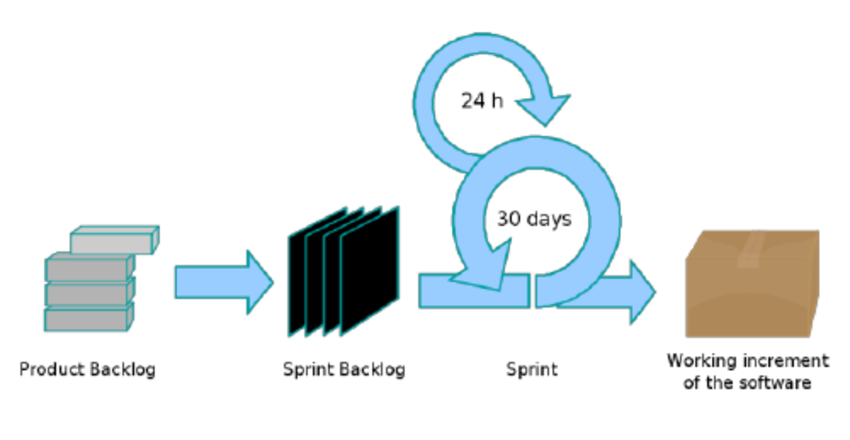
\includegraphics[scale=0.25]{img/Diagram-of-Scrum-agile-method-13.png}
\caption{Scrum process diagram \cite{inproceedings}}
\end{wrapfigure}
The approach we believed that was best suited in successfully completing our project was a Scrum approach. The Scrum approach is a software development process for smaller teams which suited us best having going from a three person team to a two person team. The breakdown of Scrum was simple to understand and put in place for this project. Like all project, the initial stage of this approach was the planning phase. This involved gathering each member and developing a structure for this project and a leading member. Mark Gill was chosen to be our project leader. His role was to outline a definitive and flexible approach broken up into what could be considered as sprints\cite{rising2000scrum}.

Sprints are short set time period in which allocated work from a project leader is completed. This work should be ready for review by the next scrum meeting. These meeting were planned and agreed upon by each member. We agreed that Monday would be a good time slot for our Scrum meeting where we reviewed work that was set out and planned for our next sprints. This day of the week was deemed to be the most optimum day as not only was it the same day as our meeting with our project supervisor, but it allowed for straightforward planning for other work we had in place from other modules for the upcoming college week. The sprints proved very effective in dividing up the work into smaller segments and setting time-frames to achieve these segments\cite{rising2000scrum}.

\section{Selection criteria for Technologies, Frameworks and Platforms}

\subsection{Technologies}
\paragraph{TypeScript}
Our initial approach included using TypeScript[1] to build our commercial application. We believed that this language was best suited for our project as it is essentially super-set of JavaScript, a language we are familiar with and have used consistently over our four years of software development. It has the ability to enable easier development on a large scale which was essential to our versatile and expandable idea\cite{bierman_abadi_torgersen_2014}.

\paragraph{Python}


\paragraph{HTML}
HTML was agreed upon for the front-end of the project. This choice was made mainly for it's simplicity. It is easily implemented and designed.

\paragraph{CSS}
CSS was agreed upon for the design of the front-end of the project. This choice was made mainly for it's simplicity.

\paragraph{JavaScript}
This choice was made mainly for it's simplicity.

\subsection{Frameworks}
\paragraph{Angular}
With our first ideas development including TypeScript, we found that Angular[] to be the best framework for our large-scale, single page application. Angular was a familiar framework to us, one that we have used for the course of two years.

\paragraph{Django}


\paragraph{Flask}


\subsection{Platforms}
\paragraph{GitHub}
As a team based final-year project, we unanimously agreed that GitHub\cite{github} would be best suited to manage our project. This decision was without hesitation as GitHub was used widely in our four years of studying Software Development. GitHub is widely used amongst every profession of software development and it is evident that the platform has helped improve the way in which software professionals work and collaborate\cite{zagalsky2015emergence}.

\section{What about validation and testing?}
Testing the application was very important to us. We wanted to ensure that it functioned smoothly and accurately. We were torn on the various ways to test our application; from using Cucumber testing, JUnit tests or the Selenium framework.

We concluded that Selenium would be the preferred testing framework to test our application.

\section{Metrics for success and failure}


\chapter{Technology Review}
This chapter will outline and breakdown each of the technologies that helped create and design this project. Each of these technologies will be discussed in detail on what they are, how they are implemented and why they were chosen over other alternative technologies.

\section{Framework}
\subsection{Django}
What it is?
How it works?
Why we chose it?

\section{Languages}
\subsection{HTML}
HTML (Hyper-Text Markup Language) is a language that makes use of tags to create web pages. These tags define which sections of the web page do what. These tags are only visible in the source code yet display cleanly on the web page when conducted correctly.

Here is an example of HTML:

Here is how the HTML is displayed:


We chose HTML as our web page display as it is extremely versatile and extensive. It is a language we have learned from our very first day of our first year of college along with CSS and JavaScript which are easily implemented with each other.

\subsection{JavaScript}
JavaScript, along with HTML and CSS, is considered a core essential for web-page design and functionality. It is said to be the backbone of any web-page and is used widely by large companies such as Google.com, Youtube.com and Facebook.com [https://w3techs.com/technologies/details/cp-javascript/]. JavaScript enables interactive web pages for the users by supporting event-driven functional programming styles such as API's.

As previously mentioned in the HTML sub-section, we chose JavaScript for our project as it was a core essential ffor the functionality of web-pages and a language we had extensive experience with throughout our college years. It enabled functionalities like our cart system in our project, something that will be detailed later in our dissertation.

\subsection{Python}



\section{Database}
\subsection{MySQL}

\section{Styling the UI}
The styling of the user interface is essentially one of the most important aspects of a web-page. Its purpose is to allow users to navigate from page to page with great ease. It is also imperative that the design is easy on the eyes of the users while still maintaining their interests by using standout colours or styles. These styles can target certain audiences in different ways. Primarily speaking, how a web-page is designed impacts how an audience will perceive a brand comparing to other competing brands.

\subsection{CSS}
CSS (Cascading Style Sheets) is primarily used to present and design markup languages like HTML. This design is achieved through improving the colours, fonts and the overall layout of a web-page.

Here is an example of a web-page with no CSS styling:

Here is the same web-page containing CSS styling:

As previously discussed in methodology, CSS was chosen for our project due to its simplicity. Along with HTML, it is a style-sheet-language we have had years of experience with and believed in using it, it would achieve our goal of an aesthetic e-commerce website.

\subsection{LaTeX}
LaTeX is a document preparation system. As opposed to the likes of Microsoft word and other word processors, LaTeX uses mark-up tags to create the structure of a document. Similarly to HTML, these tags are only visible in the source code of the document whereas it produces a a clean and concise display of the document when done correctly.

LaTeX tags are shown in this image of the source code.

% 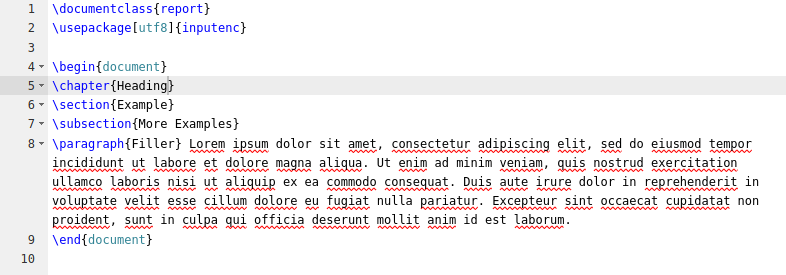
\includegraphics[scale=0.4]{img/LaTeX-Example-1.png}

This code is then compiled and can be exported to a PDF to display like the following image.

% \begin{figure}
%     \centering
%     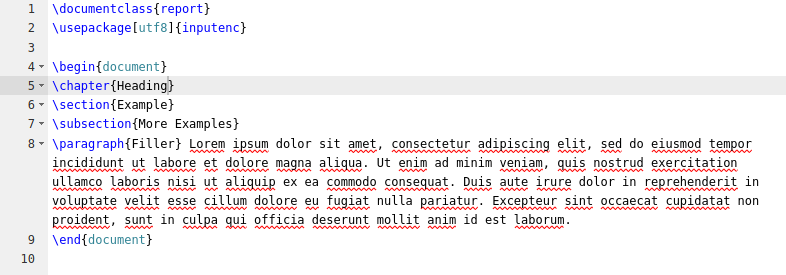
\includegraphics[scale=0.4]{img/LaTeX-Example-1.png}
%     \caption{LaTeX Output Example}
%     \label{fig:my_label}
% \end{figure}

LaTeX was the choice for our minor dissertation as we believed it was a clean and compact way of drafting up a document with the required structure put in place by our project supervisors. We were familiar with using it from a previous modules drafting documents such as literature reviews.

\newpage
\section{Integrated Development Environment}

\subsection{PyCharm}

\begin{wrapfigure}{r}{1.5in}

\includegraphics[scale=0.25]{img/PyCharm.png}
\caption{PyCharm IDE}
\end{wrapfigure}
PyCharm is an Integrated Development Environment for the Python language developed by Jetbrains. Jetbrains are a software development company targeting many fields in the software community. Their products include plugins, programming languages, team tools and many IDE's. They provide IDE's for many languages like Java, C, C++, JavaScript etc. PyCharm is cross-platform with Windows, Apples Mac and Linux operating systems. With this IDE comes many useful features. These include support for web frameworks such as Django and Flask[flask and django], integration of version control for platforms like GitHub, support for scientific tools like numpy and scipy and simplistic code navigation via clean and concise user interface.

The decision to use PyCharm was an easy one amongst our team as it was an IDE that we have been using since the beginning of our third year of software development and similar to IDE's provided by Jetbrains like IntelliJ and WebStorm which we have been using since the beginning of our second year of software development.

What we enjoy most about this IDE is it's simple and easy to use features[]. Features such as the integrated version control for committing and pushing our project to GitHub and wide support for frameworks such as Django, which is our main framework for this project, proved to be vital in aiding in stress-free coding and teamwork.
















\chapter{System Design}
As many pages as needed.
\begin{itemize}
\item Architecture, UML etc. An overview of the different components of the system. Diagrams etc… Screen shots etc.
\end{itemize}

\begin{table}[h]
  \centering
  \begin{tabular}{x{2cm}p{3cm}}
    \toprule \\
    Column 1 & Column 2 \\
    \midrule \\
    Rows 2.1 & Row 2.2 \\
    \bottomrule
  \end{tabular}
  \caption{A table.}
  \label{table:mytable}
\end{table}

\chapter{System Evaluation}
As many pages as needed.
\begin{itemize}
\item Prove that your software is robust. How? Testing etc.
\item Use performance benchmarks (space and time) if algorithmic.
\item Measure the outcomes / outputs of your system / software against the objectives from the Introduction.
\item Highlight any limitations or opportunities in your approach or technologies used.
\end{itemize}

\chapter{Conclusion}
About three pages.

\begin{itemize}
\item Briefly summarise your context and ob-jectives (a few lines).
\item Highlight your findings from the evalua-tion section / chapter and any opportuni-ties identified.
\end{itemize}

\chapter{Appendices}

\textbf{GitHub Project Source code}

\textit{\textbf{Niema Attarian:}} \href{https://github.com/niemaattarian/Final-Year-Project}{https://github.com/niemaattarian/Final-Year-Project}

\textit{\textbf{Mark Gill:}} \href{https://github.com/markgill17/Final-Year-Project}{https://github.com/markgill17/Final-Year-Project}

\textbf{Deployment link}

\textbf{Screencast of the project}